\chapter{Description générale}

\section{Environnement du projet}
Pour ce projet, je me base sur le code de mon encadrant, qui résout le sous-problème où l'ordre de réalisation des jobs et la constitution des lots sont fixés.
Le code est écrit en C++ avec Visual studio 2017 et utilise la bibliothèque Cplex.

Le projet existant utilise des fonctionnalités de Visual c++ et n'est pas compatible avec le C++ standard,
 une partie de mon travail consiste à l'adapter.
\section{Caractéristiques des utilisateurs}
Il s'agit d'un projet de recherche, les utilisateurs seront des chercheurs souhaitant tester les algorithmes développés dans ce projet.

Pour utiliser les méthodes de résolution d'instance, 
l'utilisateur doit pouvoir utiliser une invite de commande.

Pour ajouter de nouvelles méthodes de résolutions,
l'utilisateur doit disposé de Visual Studio 2017 et connaître le C++.

\section{Fonctionnalités du système}
Les applications développées dans ce projet ont pour objectif de comparer plusieurs méthodes de résolution du problème défini précédemment.
Pour cela, deux méthodes de résolutions sont testées, une méthode exacte utilisant un solveur et une recherche local.
Pour permettre de comparer les méthodes, elles utilisent la même structure de données pour les instances et les solutions.

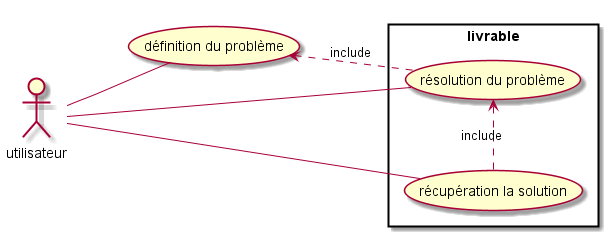
\includegraphics[width=\textwidth]{parts/description_generale/use_cases}

Les implémentations des méthodes donnent deux applications distinctes, utilisant une même bibliothèque qui définit les structures de données du problème.
Les exécutables s'exécutent en console et prennent en paramètre le chemin vers le fichier d'instance et
le chemin vers le fichier où écrire les résultats.
Les résultats sont écrits en JSON et incluent des données telles que la durée de la résolution.
L'utilisation du format JSON permet d'exploiter facilement les résultats avec de nombreux outils.


\section{Structure générale du système}



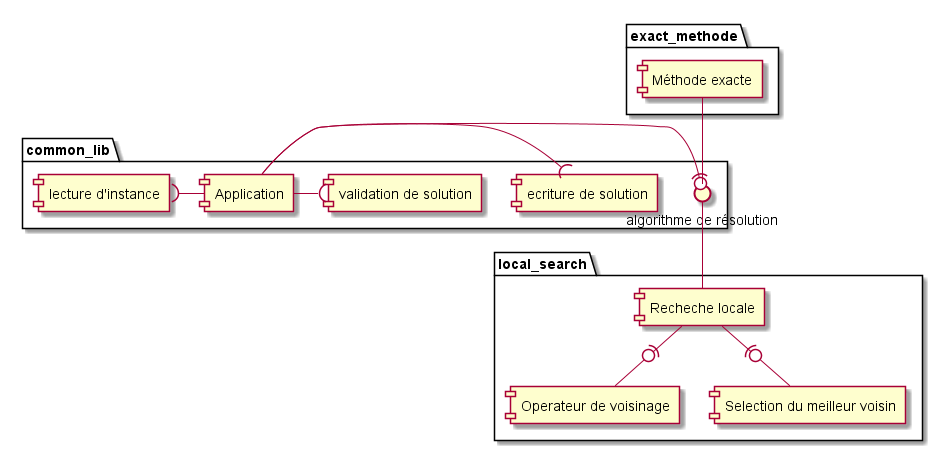
\includegraphics[width=\textwidth]{parts/description_generale/composants}

\subsection{partie commune}
Le code pour la lecture d'instance et les validations et écritures de solutions sont regroupés  dans la bibliothèque \detokenize{common_lib}.
Cette bibliothèque définit également un composant qui peut appeler et mesurer une méthode de résolution.

La bibliothèque est liée de façon statique, il n'y a pas de dll à fournir.
\subsection{Méthode exacte}

L'exécutable \detokenize{exact_methode} donne une implémentation d'une méthode de résolution utilisant le solveur CPLEX et un modèle mathématique.

\subsection{Recherche local}

L'exécutable \detokenize{local_search} implémente une méthode de résolution basée sur une recherche locale.
Les opérateurs de la recherche local peuvent avoir plusieurs implémentations.
